% !TEX root = ../main.tex
\chapter[Trazabilidad de las corridas]{Trazabilidad de las Corridas en el Almacén de Experimentos}
\label{anexo:mlflow}

La Sección~\ref{sec:experiment_tracking} describe cómo cada ejecución del sistema, sea del modo
que sea, abre una corrida de MLflow y escribe sus artefactos dentro del directorio que esa
corrida tiene asignado. Este apéndice muestra el resultado tal como lo ve quien abre el almacén,
porque es la evidencia de que las cifras que la memoria publica proceden de ejecuciones
registradas y no de un cuaderno de trabajo.

Las capturas se han tomado sobre el almacén del propio repositorio (\texttt{mlflow.db} y
\texttt{mlruns/}), navegable con \texttt{make mlflow-ui}. La
Figura~\ref{fig:mlflow_runs_table} recoge el inventario de corridas, las
Figuras~\ref{fig:mlflow_run_overview} y~\ref{fig:mlflow_run_artifacts} el detalle y los
artefactos de la que respalda el Capítulo~\ref{chap:resultados}, y la
Figura~\ref{fig:mlflow_tuning_convergence} la convergencia de una búsqueda de hiperparámetros,
que es el otro uso que el sistema hace del almacén.

\begin{figure}[H]
    \centering
    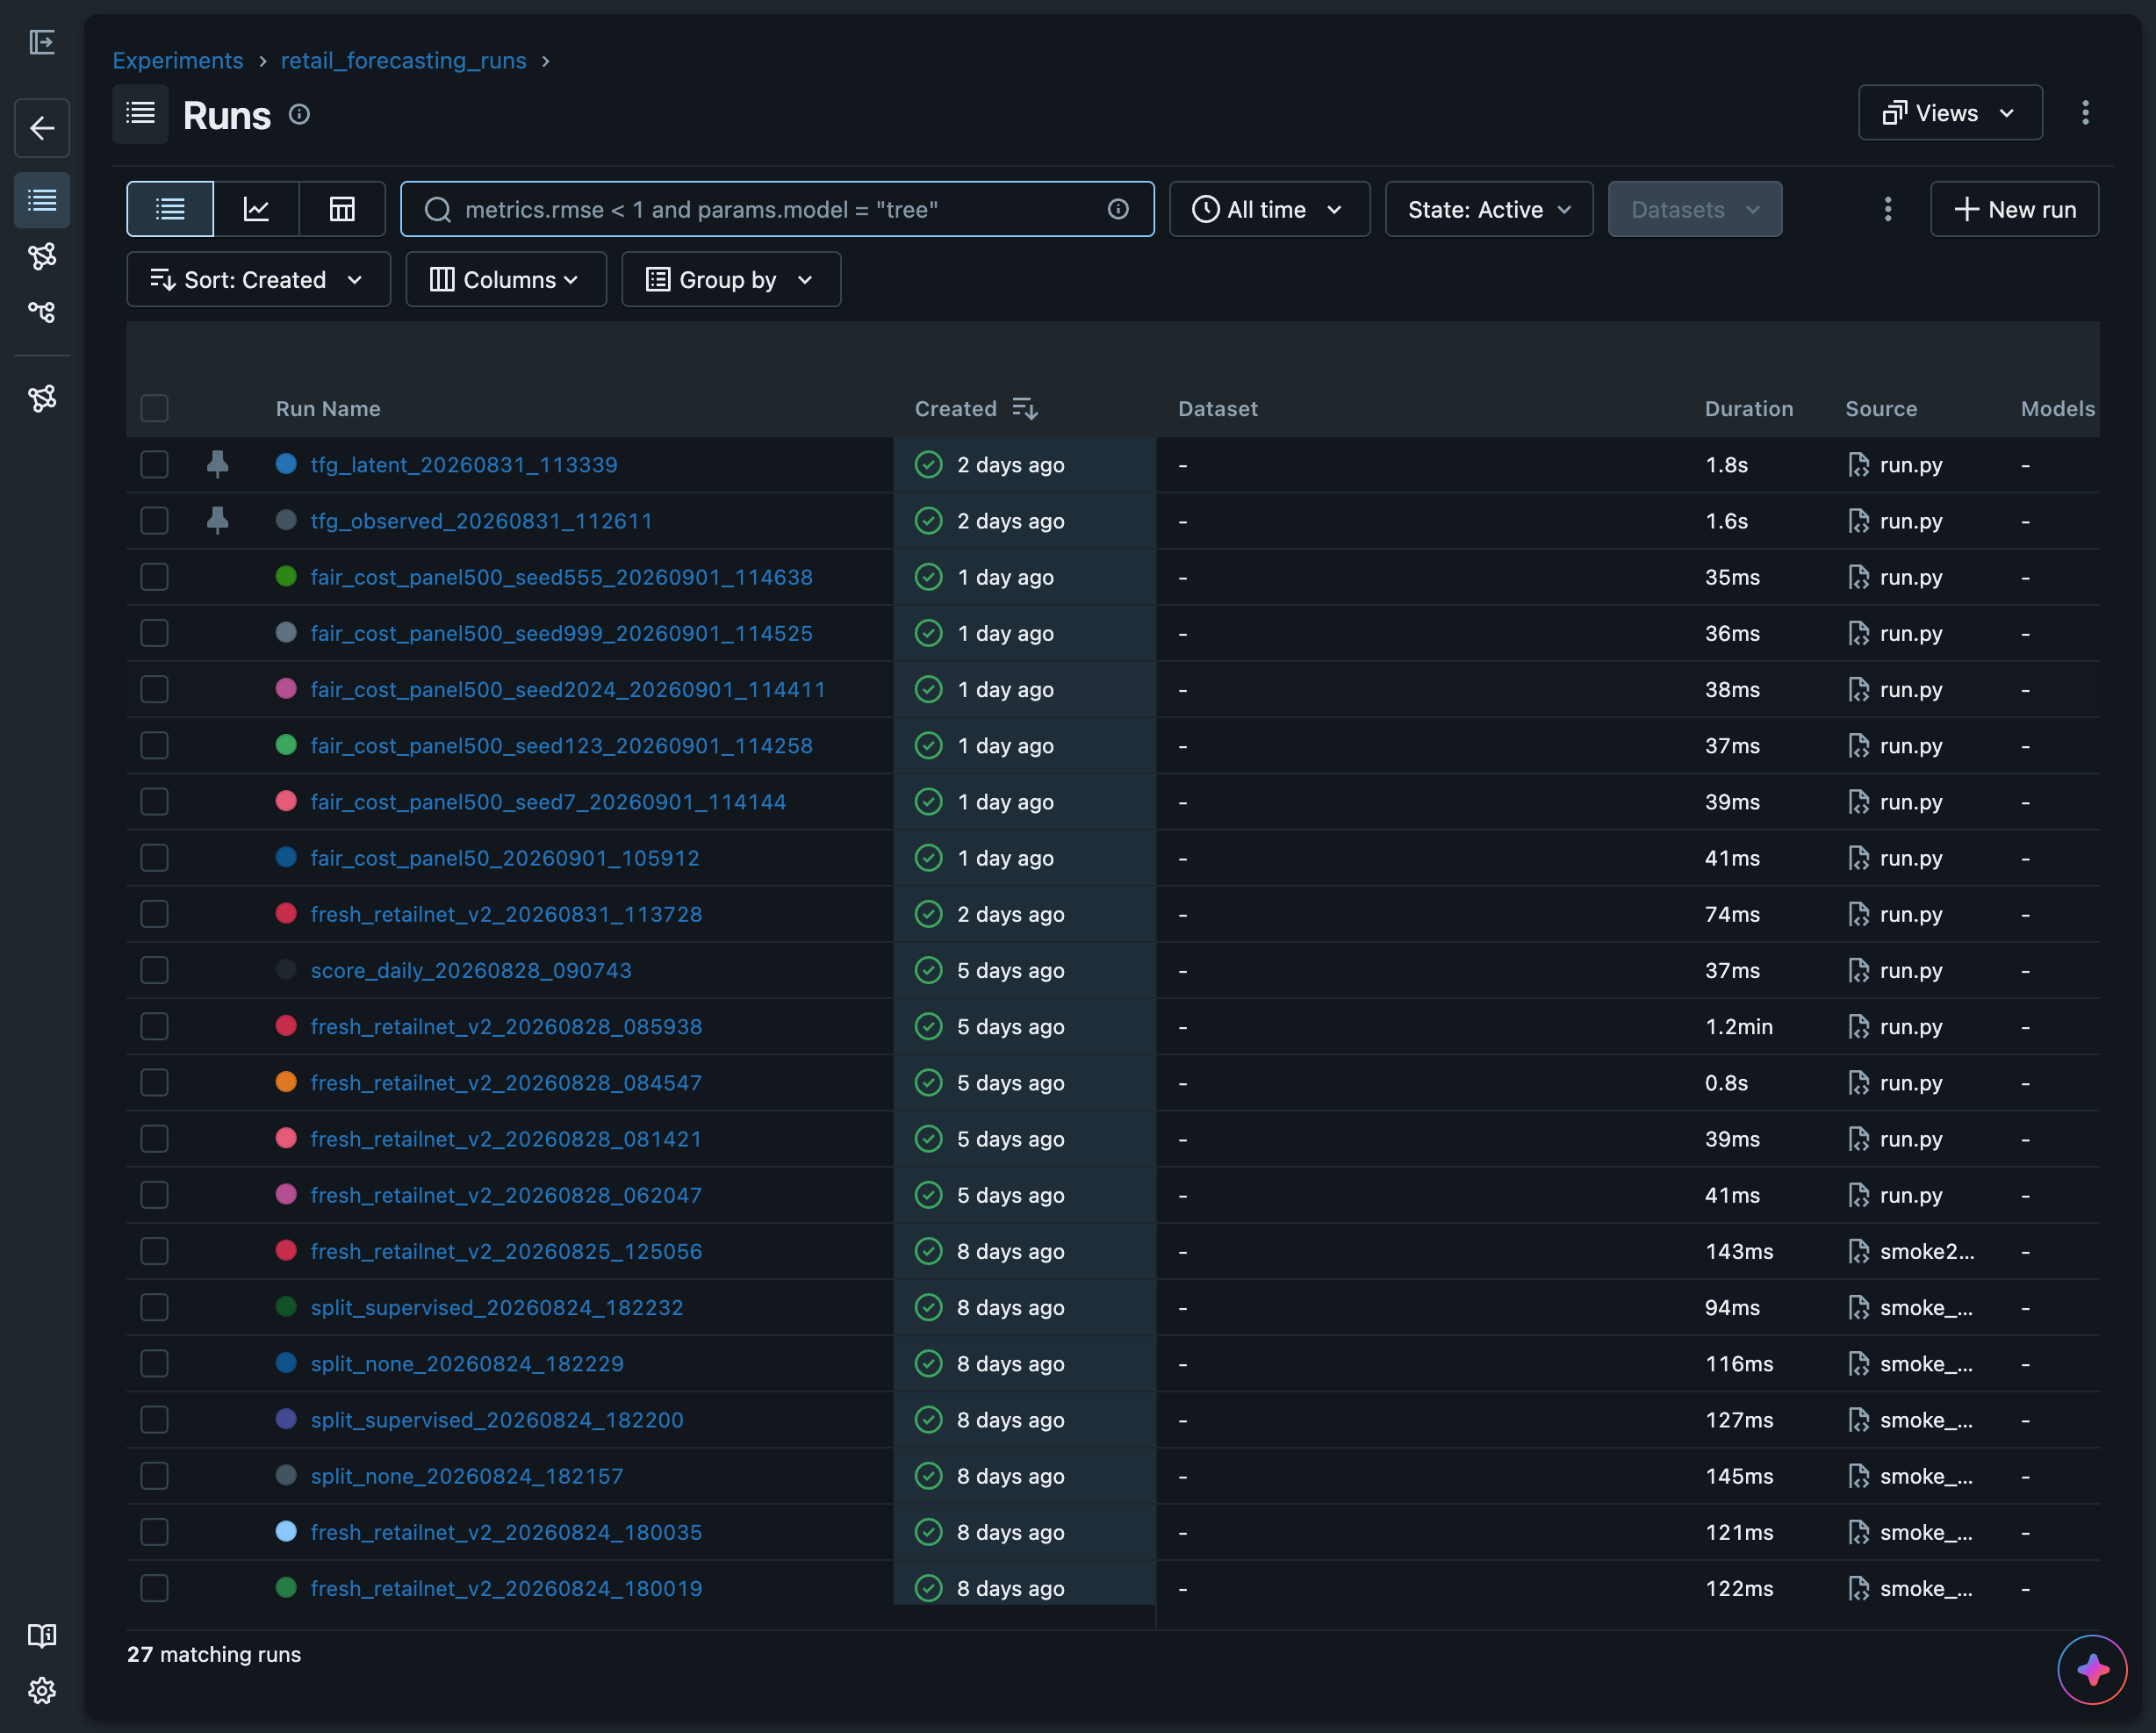
\includegraphics[width=\textwidth,height=0.80\textheight,keepaspectratio]{figures/mlflow/mlflow_runs_table.png}
    \caption[Inventario del experimento de corridas en MLflow]{Inventario del experimento \texttt{retail\_forecasting\_runs}, con 27 corridas
    registradas. Arriba, fijadas, las dos que sostienen el Capítulo~\ref{chap:resultados}:
    \texttt{tfg\_latent\_20260831\_113339} y \texttt{tfg\_observed\_20260831\_112611}. Que
    aparezcan juntas no es casual, y es lo que la Sección~\ref{sec:resultados_censura} necesita:
    son un \textbf{par emparejado} lanzado con el mismo código y la misma configuración, que
    difiere únicamente en el brazo de demanda. Debajo se distinguen las corridas del
    \textit{backtest} de coste justo, incluidas las repeticiones con distinta semilla de muestreo
    con las que se acotó la sensibilidad de la Sección~\ref{sec:resultados_gemelo}.}
    \label{fig:mlflow_runs_table}
\end{figure}

\begin{figure}[H]
    \centering
    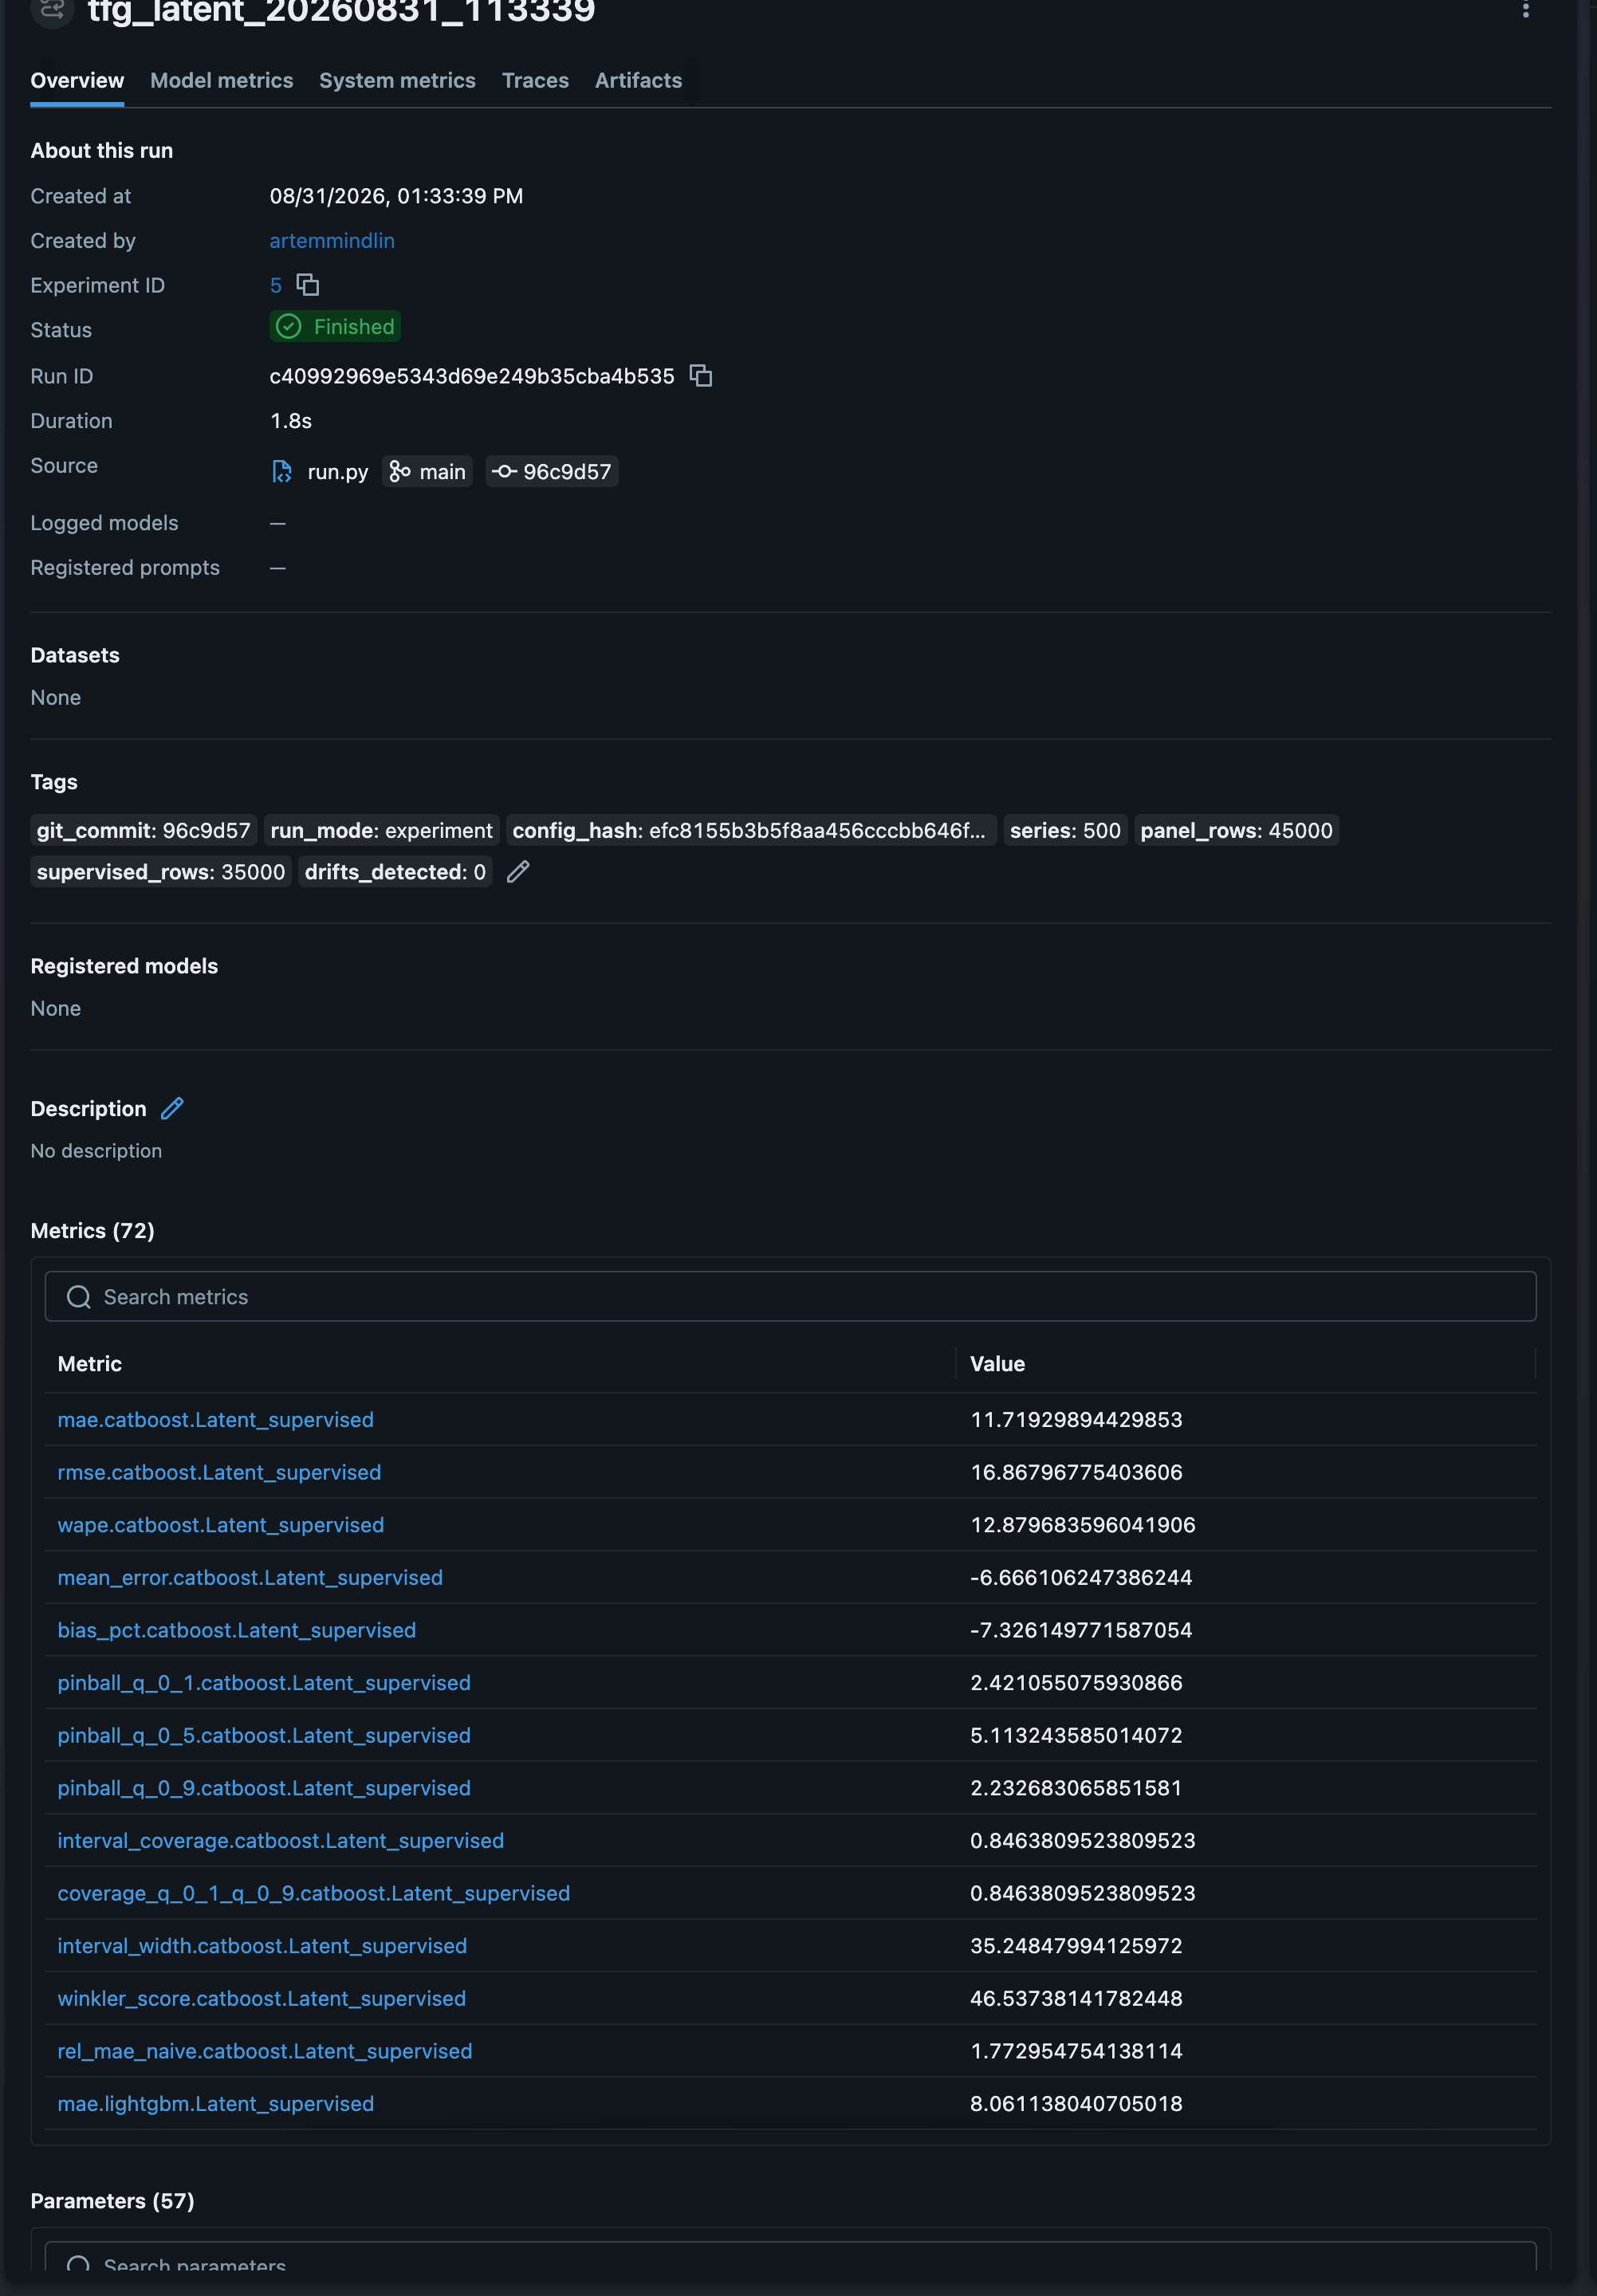
\includegraphics[width=\textwidth,height=0.80\textheight,keepaspectratio]{figures/mlflow/mlflow_run_overview.png}
    \caption[Ficha de la corrida del brazo de demanda reconstruida]{Ficha de la corrida \texttt{tfg\_latent\_20260831\_113339}, la rama de demanda
    reconstruida del experimento a 500 series. Lo decisivo para la reproducibilidad son las
    \textbf{etiquetas} de la derecha: \texttt{git\_commit} fija el código que produjo el
    resultado, \texttt{config\_hash} la configuración resuelta con la que se ejecutó, y
    \texttt{series}, \texttt{panel\_rows} y \texttt{supervised\_rows} la escala a la que se
    midió, que es el campo sin el cual dos corridas no son comparables
    (Anexo~\ref{anx:tuning_imputador}). A la izquierda, las 72 métricas indexadas por modelo y
    estrategia de datos (el MAE de CatBoost, 11{,}719, y el de LightGBM, 8{,}061, son los que
    recoge la Tabla~\ref{tab:metrics_predictive}) y los 57 parámetros de la configuración, entre
    ellos \texttt{dataset.top\_n\_series} $=500$ y \texttt{preprocessing.imputation\_strategy}
    $=$ \texttt{supervised}.}
    \label{fig:mlflow_run_overview}
\end{figure}

\begin{figure}[H]
    \centering
    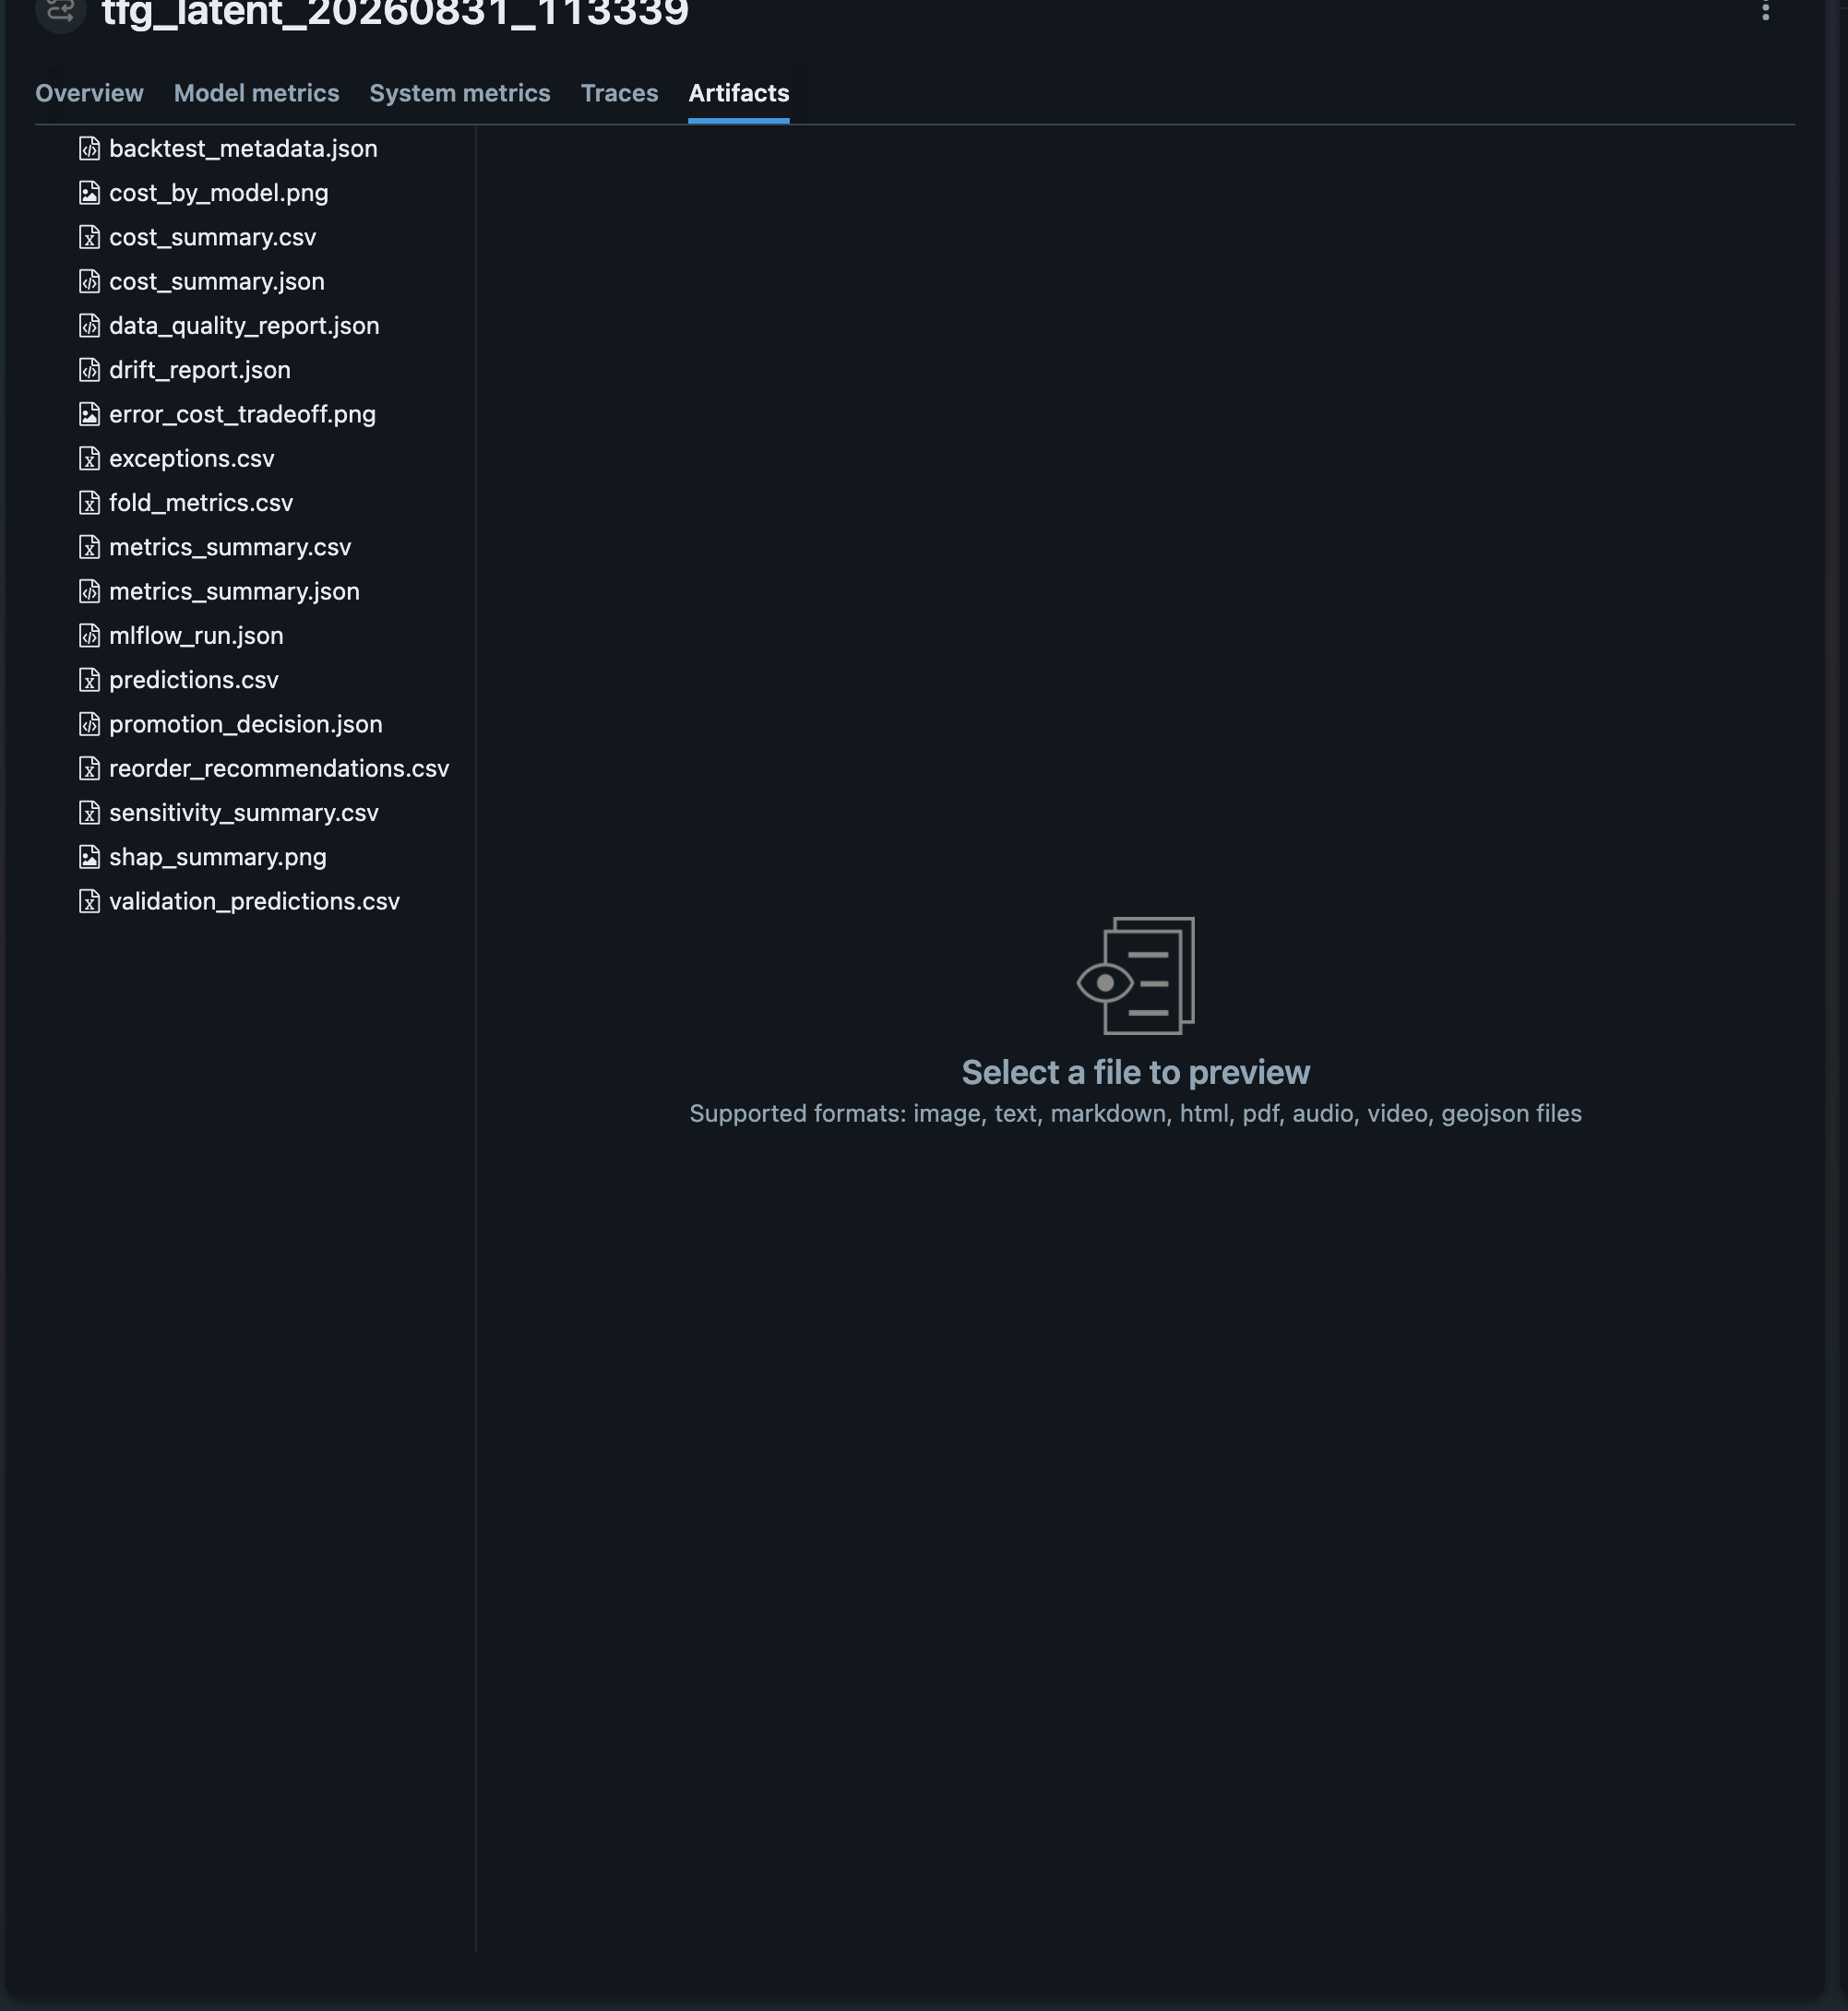
\includegraphics[width=\textwidth,height=0.80\textheight,keepaspectratio]{figures/mlflow/mlflow_run_artifacts.png}
    \caption[Artefactos de la corrida en el almacén]{Artefactos de esa misma corrida, con \texttt{predictions.csv} abierto en el panel de
    previsualización. La ruta que encabeza el panel muestra que el fichero vive dentro del
    directorio de la corrida, sin copia intermedia. En la lista conviven los dos resúmenes que el
    Capítulo~\ref{chap:resultados} explota por separado (\texttt{metrics\_summary.csv} para la
    calidad del pronóstico y \texttt{cost\_summary.csv} para la de la decisión) y los dos ficheros
    de predicciones que se computan sobre conjuntos de filas distintos: el que está abierto lleva
    una fila por origen de decisión, con su demanda objetivo a \textit{lead time} y su régimen de
    rotura. Con estos ficheros cualquier métrica publicada es recomputable sin volver a entrenar.}
    \label{fig:mlflow_run_artifacts}
\end{figure}

\begin{figure}[H]
    \centering
    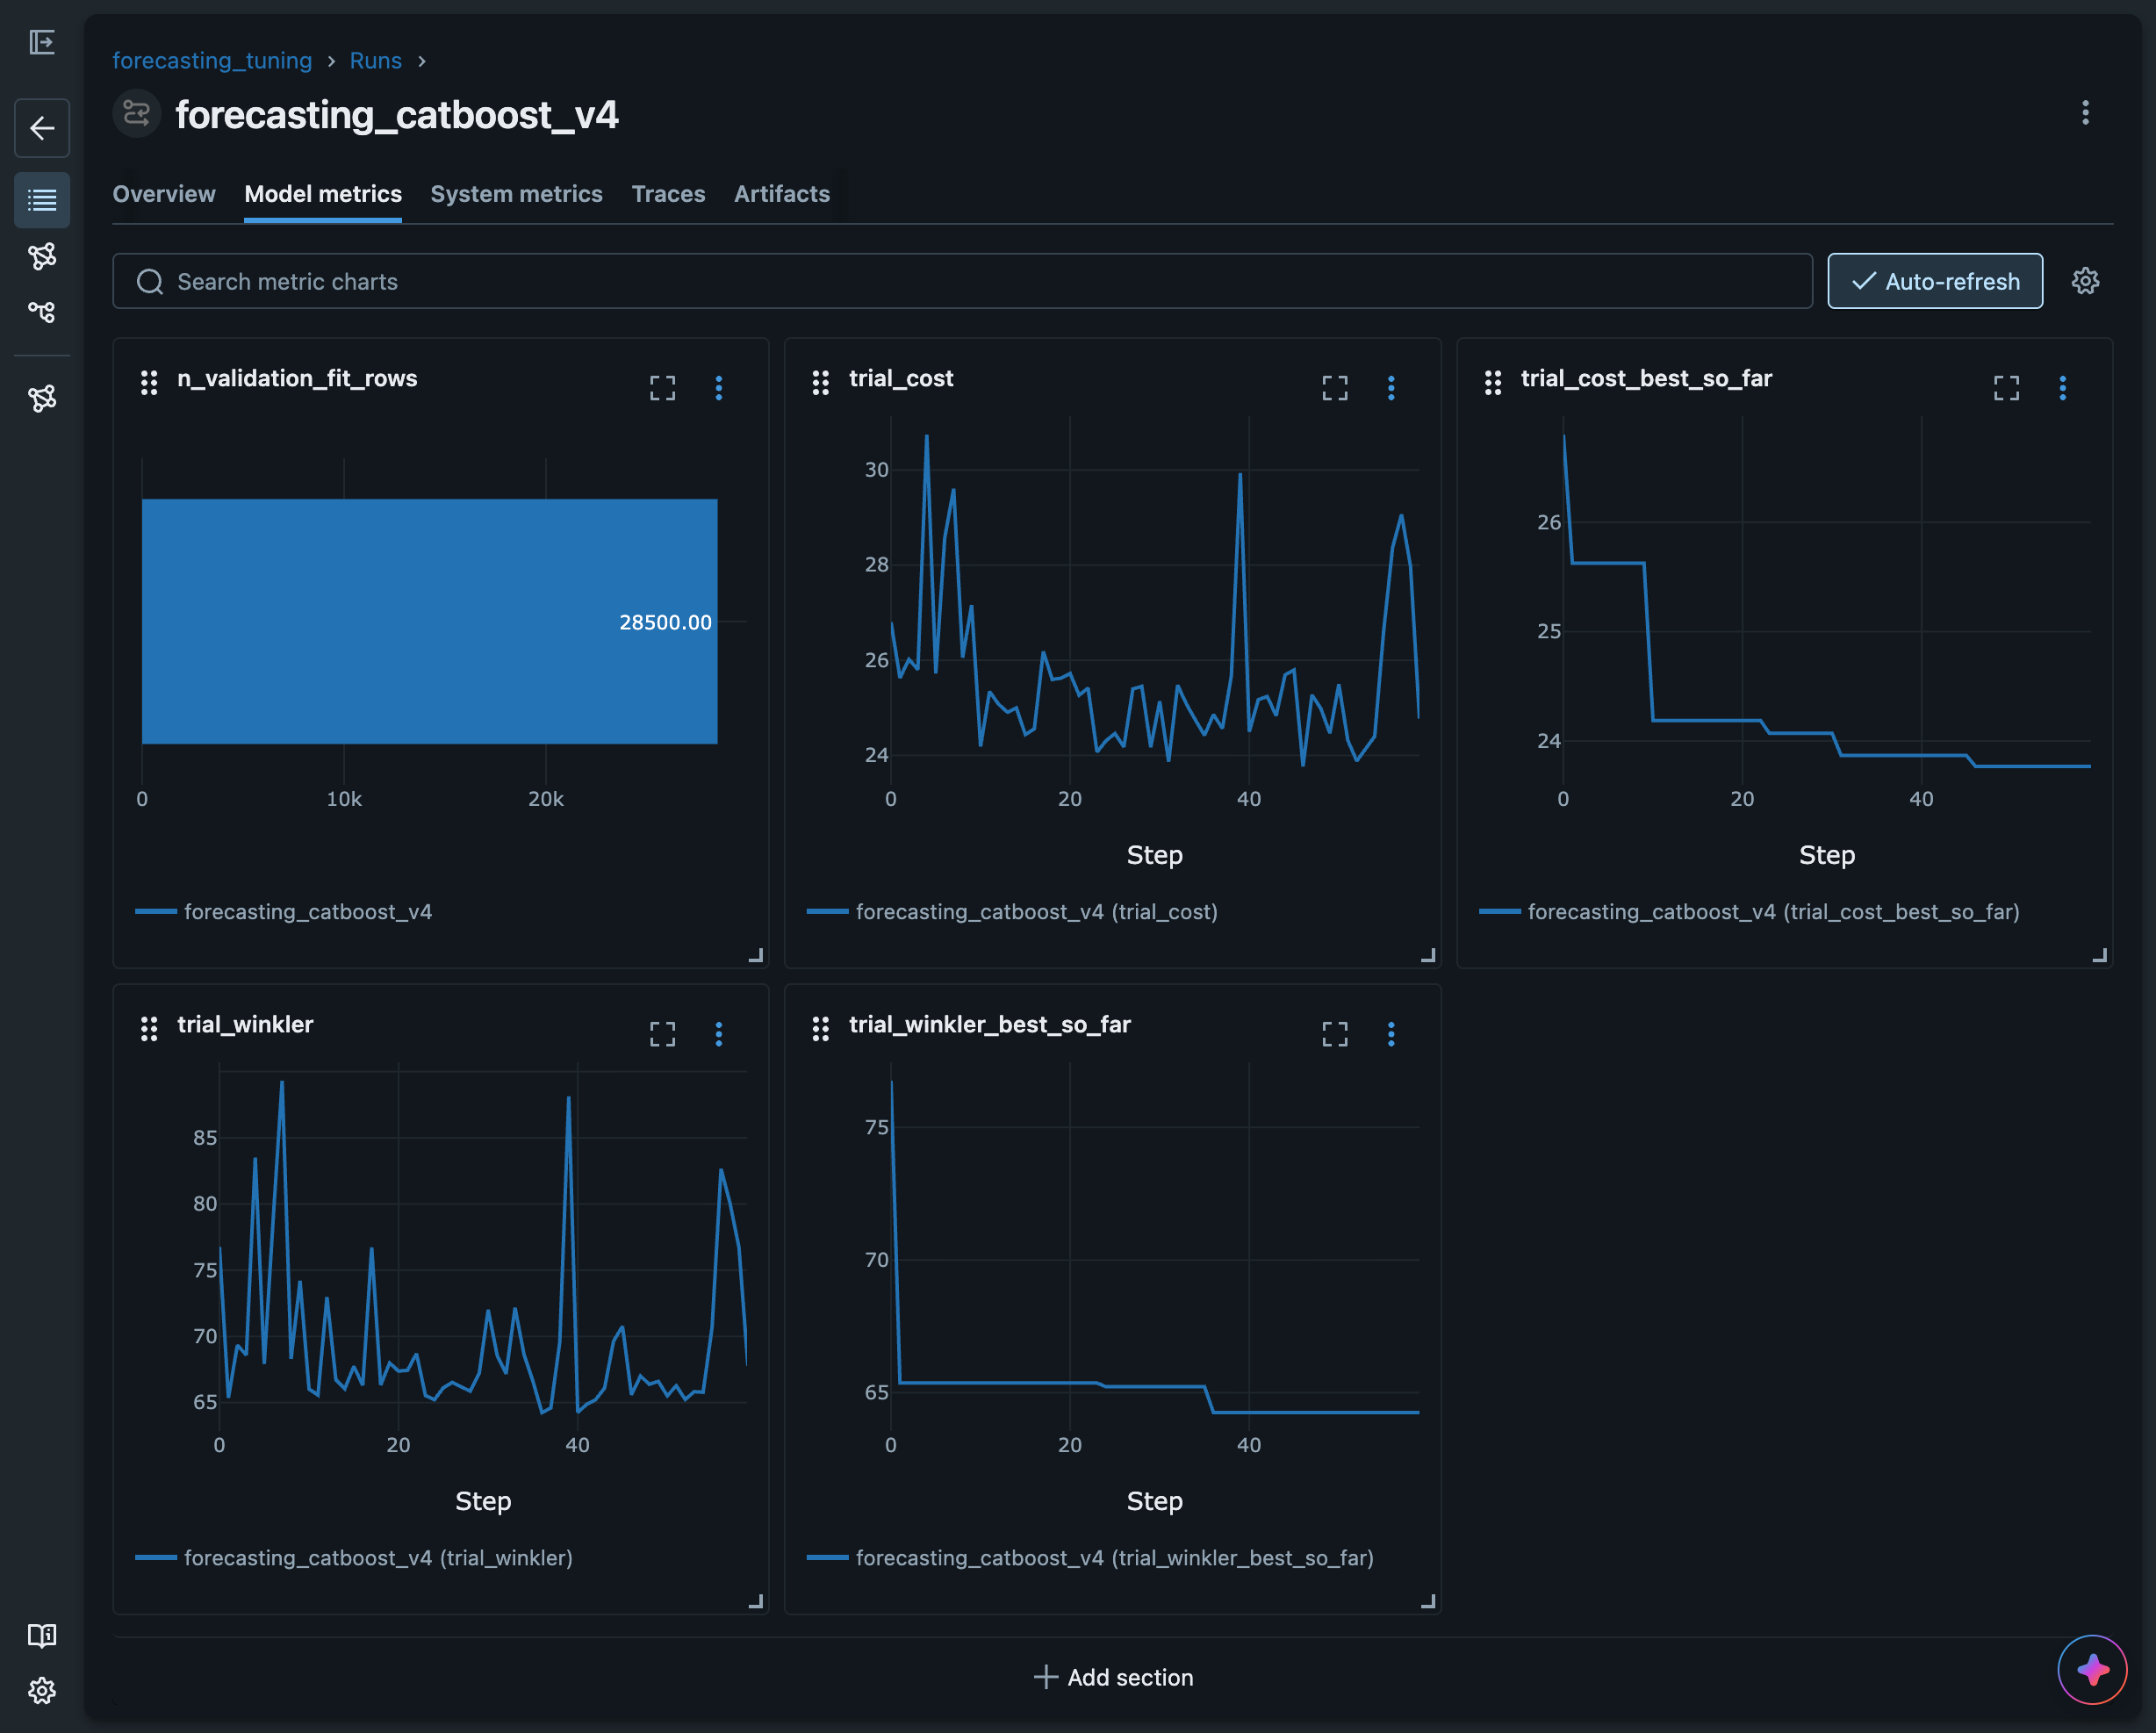
\includegraphics[width=\textwidth,height=0.80\textheight,keepaspectratio]{figures/mlflow/mlflow_tuning_convergence.png}
    \caption[Métricas de la búsqueda de hiperparámetros de CatBoost]{Métricas registradas por la búsqueda de hiperparámetros
    \texttt{forecasting\_catboost\_v4}, en el experimento \texttt{forecasting\_tuning}. Las dos
    gráficas de la derecha son las que importan y hay que leer juntas: \texttt{trial\_cost} da el
    coste de cada uno de los 60 \textit{trials}, que oscila sin tendencia entre 24 y 30, mientras
    que \texttt{trial\_cost\_best\_so\_far} da el mejor acumulado, que desciende a saltos y se
    estabiliza pasado el \textit{trial} 40. La dispersión entre \textit{trials} es del orden de la
    mejora total de la búsqueda, que es exactamente la observación con la que el
    Anexo~\ref{anx:tuning_imputador} justifica promediar sobre múltiples extracciones en lugar de
    fiarse del valor objetivo de un \textit{trial} suelto.}
    \label{fig:mlflow_tuning_convergence}
\end{figure}
